\documentclass[12pt,a4paper]{report}
%====================== PACKAGES ======================
\usepackage[utf8]{inputenc}
\usepackage[arabic,french]{babel}
\usepackage[LAE,T1]{fontenc}
%Line break after paragraphes 
\usepackage[raggedright]{titlesec}
\titleformat{\paragraph}[hang]{\normalfont\normalsize\bfseries}{\theparagraph}{1em}{}
\titlespacing*{\paragraph}{0pt}{3.25ex plus 1ex minus .2ex}{0.5em}
%Accronym
\usepackage[french]{nomencl}
% Load the package
% Load the package with the acronym option
 


%Mis en page :
\usepackage{lastpage}
\usepackage[top=2cm, bottom=2cm, left=2cm, right=2cm]{geometry}
\usepackage[Glenn]{fncychap}
\usepackage{fancyvrb}
\usepackage{fancyhdr}
\setlength{\headheight}{13.1pt}
 
\fancyhead[]{}
\lhead{\leftmark}
\cfoot{}
\fancyfoot[R]{\thepage}
% Redefine the plain page style
\fancypagestyle{plain}{%
\fancyhead[]{}
\lhead{\leftmark}
\cfoot{}
\fancyfoot[R]{\thepage}
}

%Biblio
\usepackage{pdflscape}
\usepackage{afterpage}
\usepackage[authoryear]{natbib}
\usepackage{hyperref}
\hypersetup{
	colorlinks,
	citecolor=blue,
	filecolor=black,
	linkcolor=black,
	urlcolor=black
}

%Images and figures
%\usepackage{setspace}
\usepackage{graphicx}
\graphicspath{ {Resources/} }
%Page de garde
\usepackage{framed}
%Rotating
\usepackage{rotating}
%\usepackage{tikz}
\newcommand*\rot{\rotatebox{90}}
%Math using equations
\usepackage{amsmath,amsfonts,amssymb}
%pour gérer les positionnement d'images
\usepackage{float}
%caption
\usepackage[caption=false]{subfig}

\captionsetup[table]{aboveskip=10pt}
\captionsetup[table]{belowskip=10pt}
\captionsetup{justification=centering}
\captionsetup[table]{name=Tableau}
%Toc

%Tables
\setcounter{secnumdepth}{5}
\usepackage{tabularx}
\usepackage{chngcntr}\counterwithout{figure}{chapter}
\usepackage{chngcntr}\counterwithout{table}{chapter}
\renewcommand{\thetable}{\Roman{table}}
%page de garde
\usepackage{pdfpages}
\hypersetup{							% Information sur le document
	pdfauthor = {KEBAILI Zohra Kaouter,
		KECHIDA Fatima Zahra,
	},			% Auteurs
	pdftitle = {Plateforme de test multicritères adapté aux solutions
		multi-biométriques},			% Titre du document
	pdfsubject = {Mémoire de Projet},		% Sujet
	pdfkeywords = {Tag1, Tag2, Tag3, ...},	% Mots-clefs
	pdfstartview={FitH}}					% ajuste la page à la largueur de l'écran
\begin{document} 
	%page de garde
	%====================== INCLUSION DES PARTIES ======================
	%
\begin{titlepage}
 \begin{center}
 
\includegraphics[scale=0.9]{Others/Resources/entete.png}\\
 \vspace*{1cm}
  \LARGE
  \textbf{Rapport du Master\\}
  \large
 
  \LARGE
  	\vspace{2cm}
  \textbf{Option: Systèmes et ingénierie de logiciels}\\
  \vspace{1cm}
  \LARGE
  \textbf{Thème}\\
  \vspace{1cm}
  \LARGE
  \setlength{\fboxsep}{0.5cm}
  \begin{framed}
	\textbf{Les anti-patrons linguistiques}
  \end{framed}
  \vspace{2cm}
  \begin{table}[H]
   \setlength{\tabcolsep}{2cm}
    \large
	\centering
	\begin{tabular}{ll}
		\textbf{Réalisé par :}    
		 & \textbf{Encadré par : } \\  \\
		 -\textsc{Mlle Kebaili} Zohra Kaouter 
	
	& -\textsc{ Mme Bousbia} Nabila   \\
	

	\end{tabular}
  \end{table}
  \vspace{\fill}
  \large
  \textbf{Promotion 2017/2018}
        
 \end{center}
\end{titlepage}
	\includepdf{Page_garde}
     \pagenumbering{Roman}
     \pagestyle{fancy}
	\setcounter{page}{2}

\addcontentsline{toc}{chapter}{\contentsname}
\tableofcontents

\addcontentsline{toc}{chapter}{\listfigurename}
\listoffigures

\addcontentsline{toc}{chapter}{\listtablename}
\listoftables

 \chapter*{Liste des sigles et abréviations}
 \addcontentsline{toc}{chapter}{Liste des sigles et abréviations}
 \printnomenclature
	\chapter*{Liste des sigles et abréviations}% Main chapter title
\begin{table}[H]
	\label{my-label}
	\begin{tabular}{ll}
		\textbf{API} & Application Programming Interface    \\
		\textbf{AST}   & Arbre Syntaxique Abstrait                          \\
		\textbf{CBO}  & Coupling Between Objects                \\
		\textbf{IR}  & Information Retrieval                 \\
		\textbf{LOC}  & Ligne Of Code                     \\
		\textbf{LSI}  & Latent Semantic Indexing                    \\
		\textbf{NL}  & Natural Language               \\
		\textbf{OO} & Orienté Objet \\
			\textbf{RESTful} & REpresentational State Transfer \\
			\textbf{SOA} & Architecture Orientée Service \\
			\textbf{SQL} & Structured Query Language \\
		\textbf{SVM} & Machines à Vecteurs de Support                \\
		
		\textbf{SP}   & Singulier Points                        
	\end{tabular}
\end{table}

	\chapter*{Introduction générale}
%\section{Introduction}
\tab Avec le développement logiciel continu et rapide, un programme subit beaucoup de changements pendant son cycle de vie, ce qui engendre des fautes suite à des mauvaises habitudes exercées par les développeurs sous pression ou par ignorance. Ces mauvaises pratiques affectent la qualité logicielle et rend difficile la compréhension du code que ce soit par l’auteur du code lui même après quelques modifications ou bien par d’autres développeurs lors de la maintenance. Cette dernière avec ses types: Corrective, préventive, adaptative et  perfective, représente une activité inévitable lors du développement logiciel et vise à produire un logiciel de qualité.  
\vspace{5px}\\
Pour améliorer la qualité logicielle, plusieurs techniques existent, parmi ces techniques: l’utilisation de l’information linguistique, l’utilisation des bons identificateurs, la bonne documentation et l’utilisation du bon lexique. C’est pourquoi, de nouveaux travaux de recherches sont apparus pour exploiter l’information linguistique d’un programme pour identifier les mauvaises pratiques liées au coté linguistique d’un programme ce qui a mené à l’apparition des «Lexicon bad smells» et des «anti-patrons linguistiques». 
\vspace{5px}\\
L’objectif de ce rapport est de comprendre ce que c'est un lexicon bad smell, que c'est un anti-patron linguistique, les lexicon bad smells et les anti-patrons linguistiques connus jusqu’à maintenant et comment les détecter.
     \pagenumbering{arabic}	
	
\chapter{Généralités}
\section{Introduction}
Une conception parfaite dès le premier coup n’existe pas, ce qui fait de la tâche de conception une tâche itérative. Les concepteurs avec l’expérience ont remarqué qu’il y a quelques choses qui se répètent d’une conception à l’autre, ce qui a donné naissance à la notion de « patron » et « anti patron » de conception.
\vspace{5px}\\
Dans ce chapitre, nous présentons les patrons et les anti-patrons de conception et nous citons les approches utilisées pour détecter ces anti-patrons.

\section{Les patrons de conception}
La notion de patron de conception est apparue avec les travaux de \cite{alexander1977pattern} dans le domaine d’architecture, et depuis, ce même concept a été appliqué dans le domaine de gestion de projet et de la conception de logiciels informatique à laquelle nous nous intéressons dans ce rapport. \newline
Les patrons de conception orientée objet ont été popularisés avec la publication en 1994 du livre : Design Patterns : Elements of Reusable Object Oriented Software \cite{vlissides1995design} qui est un catalogue de patrons de conception indépendant du langage de programmation. \newline
Un patron de conception est défini comme étant une solution générale à un problème récurrent dans un contexte particulier. Un patron de conception est décrit avec quatre éléments \cite{vlissides1995design}:
\newline
\begin{itemize}
   

  \item Le nom du patron : qui peut repérer le problème et la solution, est le moyen de communication entre les développeurs concernant ce patron.
  \item Le problème : décrit le contexte ou la situation dans laquelle le patron s’applique.
  \item La solution : décrit les éléments de la conception qui règlent le problème détecté, indépendamment de l’implémentation et du langage, qui peut être utilisée dans d’autres situations.
  \item Les conséquences : décrit les résultats de l’application du patron et son impact sur la flexibilité et l’extensibilité de la solution.
\end{itemize}
\newline
Les patrons de conception sont catégorisés sous trois types selon leur mission :
\begin{itemize}
    \item Patrons de création: Exemples; Abstract Factory, Builder, Factory.
    \item Patrons de comportement: Exemples; Adapter, Bridge, Composite.
    \item Patrons de structure: Exemples; Interpreter, Iterator, Mediator.
\end{itemize}
\section{Les anti-patrons de conception et les code smells}
Ce terme introduit pour la première fois par Koenig en 1998, veut dire les mauvaises solutions récurrentes à des problèmes de systèmes logiciels \cite{brown1998antipatterns}. Il est important pour les développeurs de connaître les anti-patrons, pour savoir les situations où une solution peut avoir un impact négatif et donc l’éviter, parmi les anti-patrons les plus connus, nous citons: Blob, Spaghetti Code, Swiss Army Knife.
\newline
Afin de détecter les anti patrons, des symptômes ont été recensés, appelées, code bad smells, qui représentent des signes de manifestation dans le code source qui aident à mieux trouver les parties de code pouvant contenir des anti-patrons.
\newline
Ils sont catégorisés selon \cite{mantyla2003taxonomy} sous six groupes (sauf deux smells qui ne rentrent dans aucun groupe qui sont: Incomplete Library Class et Comments) afin de comprendre la relation entres les code smells de même groupe et trouver les corrélations entre eux pour optimiser l'étape de refactoring:
\begin{itemize}
    \item \textbf{The Bloaters} : englobent les code smells qui caractérisent les classes et méthodes qui sont très grandes et difficilement maintenables, par exemple: Long Method, large class qui implique l’existence de l’anti-patron Blob, Primitive Obsession ou Long Parameter List.
    \item \textbf{The Object-Oriented Abusers} : englobent les code smells qui caractérisent des cas où les principes orientées objet ne sont pas respectés (polymorphisme, encapsulation...etc.) par exemple: Switch Statement qui peut être transformé en exploitant le polymorphisme, le bad smell Poor Usage of Abstract Classes.
    \item \textbf{The Dispensables} : englobent les code smells qui caractérisent les classes supplémentaires, qui ne jouent presque aucun rôle dans le code, par exemple :Lazy Class,Data Class
    \item \textbf{The Couplers} : ce sont les défauts de conception qui augmentent le couplage entre les classes, exemples :Law of Demeter
    \item \textbf{The Encapsulators} : englobent les code smells qui ont une relation avec les mecanismes de communication et d'encapsulation des données dans le code source, par exemple, le code smell Message Chains .
    \item \textbf{The Change Preventers} : englobent les code smells qui impliquent, en cas de modification dans le code source, que soit une classe doit être modifiée suite à plusieurs types de modification comme le code smell Divergent Change ou bien plusieurs classes à modifier au cas d'un seul changement comme le code smell Shotgun Surgery, parce que , les modifications possibles doivent avoir une relation 1-1, c'est à dire, un seul changement implique la modification d'une seule classe.
\end{itemize}
\vspace{1cm}
La compréhension des causes d'apparition des anti-patrons est aussi importante que son étude, c'est pourquoi, nous citons ici les causes principales qui peuvent engendrer un anti-patron de conception\cite{brown1998antipatterns}:

\begin{itemize}
\item  La conception sous des contraintes de temps : le but dans ce cas est de réaliser quelque chose de fonctionnel, mais pas nécessairement maintenable ou de qualité.
\item Le changement continu du code : sans comprendre le code surtout par des développeurs différents de ceux qui ont écrit le premier code source.
\item Le non-respect des bonnes pratiques de conception et de codage.
\item L’ignorance et/ou la fierté des développeurs : ne pas commenter son code ou ne pas bien écrire ses commentaires est l'un des exemples les plus simples de ce cas.
\end{itemize}
\vspace{1cm}
Un autre aspect à aborder concernant les anti-patrons, c'est la documentation, qui est très importante pour permettre la communication facile entre les développeurs, et comme les patrons, les anti-patrons ont leur propre documentation aussi qui figure sous plusieurs formes :
\begin{itemize}
    

    \item \textbf{La pseudo-documentation}: donne le nom et le problème de l’anti-patron en question.
    \item \textbf{La mini-documentation }: fournit le nom de l’anti-patron, le problème et la solution proposée.
    \item \textbf{La documentation complète}: contient le nom le plus connu, les autres noms s’il en existe, contient aussi le niveau fréquent auquel  cet anti-patron peut être détecté(niveau application,micro architecture ou framework..etc) , le nom de la solution et son type, les forces déséquilibrées qui ont été sous-estimées comme la gestion de fonctionnalités ou gestion de complexité, la forme générale de l’anti-patron donnée sous forme de diagramme, symptômes et conséquences, aussi les exceptions connues où cet anti-patron n’a pas d’impact négatif, d’autres anti-patrons liés à l’anti-patron en question, exemple et applicabilité à d’autres niveaux.
\end{itemize}
\vspace{1cm}
Dans la figure \ref{fig:patanti} ci-dessous, \cite{brown1998antipatterns} illustre la relation entre les patrons et les anti-patrons.

\begin{figure}[H]

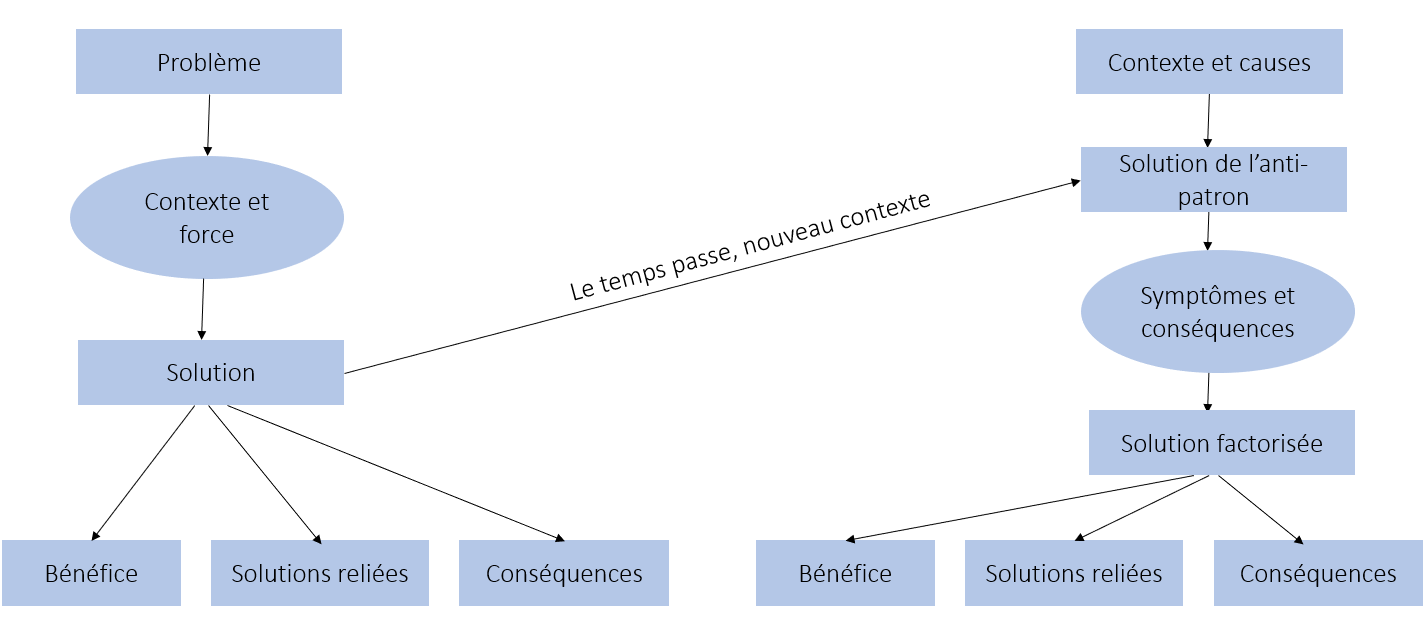
\includegraphics[width=\textwidth]{Others/Resources/patronetantipatron.PNG}
	\caption{La relation entre les patrons et les anti-patrons \cite{brown1998antipatterns}.}
		\label{fig:patanti}
	\end{figure}
	
	\section{Détection  des anti-patrons de conception}
	Dans ce paragraphe, nous présentons brièvement les différentes approches de détection des anti-patrons qui existent déjà dans la littérature.
	
	\cite{travassos1999detecting} ont introduit un processus basé sur les inspections manuelles et les techniques de lectures afin d’identifier les mauvaises odeurs du code. Aucune tentative n'a été réalisée pour automatiser ce processus, et par conséquence, la technique resterait difficilement applicable sur les systèmes logiciels compliqués.
\cite{marinescu2004detection} a présenté une approche basée sur les métriques pour détecter les odeurs de code avec des stratégies de détection. Cette approche est mise en œuvre via l'outil IPLASMA. La stratégie consiste à capter à l'aide des métriques, les écarts par rapport aux bons principes de conception, ensuite elle combine ces métriques avec des opérateurs  et compare leurs valeurs par rapport à des seuils absolus et relatifs.
\cite{munro2005product} a remarqué les limitations des descriptions textuelles et a proposé un modèle pour décrire les odeurs de code systématiquement. Ce modèle est similaire à celui utilisé pour les patrons de conception \cite{vlissides1995design}. Il se compose de trois parties principales : le nom de l'odeur de code, la description textuelle de ses caractéristiques et les heuristiques utilisées pour sa détection.
\newline
Ce travail est considéré comme un pas vers des spécifications plus précises des odeurs de code. Munro a également proposé des heuristiques basées sur les métriques pour détecter les odeurs de code, qui sont similaires aux stratégies de détection de Marinescu. Il a également effectué une étude empirique pour justifier le choix des métriques et des seuils de détection des odeurs.
\newline
\cite{alikacem2009metric} ont proposé un langage pour détecter les violations des principes de qualité et des odeurs dans les systèmes orientés objets. Ce langage permet la spécification de règles en utilisant les statistiques, l'héritage ou les relations d'association entre classes, selon les attentes des ingénieurs. Il permet également d'utiliser la logique floue (fuzzy logic) pour exprimer les seuils de règles conditions qui sont exécutées par un moteur d'inférence. Quelques approches traitant les systèmes complexes utilisent les techniques de visualisation \cite{dhambri2008visual}, \cite{simon2001metrics}, telle que les approches semi-automatiques qui sont intéressantes comparées avec les techniques automatiques qui peuvent être efficaces  mais perdent la trace du contexte et l'inspection manuelle est lente et inexacte \cite{langelier2005visualization}, de plus, elle
nécessite une expertise humaine et donc encore plus de temps. 
\newline
D'autres approches de détection fonctionnent entièrement d’une façon automatique pour détecter des odeurs de code et utilisent les techniques de visualisation pour présenter les résultats de la détection \cite{lanza2007object}, \cite{van2002java}.
D'autres approches connexes incluent les détecteurs de cohérence architecturale, qui ont été intégrées dans les environnements architecturales de développement \cite{garlan1995architectural}, \cite{allen1997formal},\cite{dashofy2005comprehensive}.
Par exemple, les agents actifs agissant comme des critiques \cite{dashofy2005comprehensive} qui peuvent vérifier les propriétés des descriptions architecturales, identifier les erreurs syntaxiques et sémantiques potentielles et les signaler au concepteur.
Toutes ces approches ont contribué d’une manière significative à la détection automatique des odeurs. 

	\chapter{Les anti-Patrons linguistiques }
Dans le chapitre précédant, nous avons expliqué ce que c'est un patron de conception  et ce que c'est un anti-patron de conception ainsi que les approches connues de détection des anti-patrons.
  \vspace{5px}
Dans ce chapitre, nous nous intéressons à une classe bien particulière des anti-patrons qui est les anti-patrons linguistiques, nous commençons par comprendre c'est quoi un lexicon bad smells et puis expliquer la notion d'anti-patron linguistique.
\section{La relation entre le lexique du code et sa qualité }
Le réglage des bugs dans les logiciels en cours de production est une tache très coûteuse en terme de temps et d’argents pour les entreprises, c’est pourquoi, 
les développeurs, donnent une grande importance à la tache de test pour identifier les classes pouvant causer des bugs dans le futur (faulty classes) 
et atteindre le but de prédire quelles classes sont plus exposées à causer des bugs (ie Faulty classes prédiction). Pour supporter la tache de test, qui a pour finalité, 
d’améliorer la qualité logicielle, des recherches ont été menées pour mesurer la qualité logicielle. Ces recherches portent sur plusieurs axes, parmi ces axes: 
les métriques structurales, les métriques des processus (process metrics), et les fautes précédentes(previous faults)\cite{abebe2012can}.
\newline
Les métriques structurales sont largement utilisées( comme par exemple DIT :depth of inheritance tree et CBO : coupling between objects), car le code est complexe et difficile à comprendre, et pour éviter d’y entrer, il est utile d’avoir des informations concernant la structure générale de ce code.
\newline
D’autre part,il y a des recherches qui donnent de l’importance aux identificateurs, \cite{haiduc2008use}, \cite{butler2009relating}, et le lexique du code sources qui peut largement influencer la compréhensibilité du code( documentation insuffisantes, convention de nomination différente et pas nécessairement toujours suivie), le code peut être lu par d'autres personnes autres que ceux qui l’ont écrit, testeurs différents des codeurs, changement des employés, remplacements et bien d'autres situations, donc, ça sera très bénéfique d’améliorer le lexique du code, pour augmenter sa compressibilité et donc améliorer les tests pour  améliorer la qualité logicielle par la suite\cite{abebe2012can}.
\newline
Pour atteindre ce but, il vaut mieux améliorer la qualité du lexique utilisé dans le code source.
\newline
 \vspace{5px}
A partir de ce constat, des études ont été menées pour cerner les différentes fautes concernant le lexique(choix d’identificateurs, noms de classes, termes utilisés dans les commentaires..etc) pour les éviter.
D’où la naissance du Lexicon Bad smells et les anti patrons linguistiques.
\section{Lexicon Bad Smells }
\label{lbs}
Dans ce paragraphe, nous présentons les différents lexicon bad smells trouvés dans la littérature qui peuvent être utiles dans la prédiction des anti-patrons linguistiques ou même peuvent être considérés comme des anti-patrons linguistiques, pour pouvoir citer les algorithmes de détection plus tard dans ce rapport, nous les représentons en suivant un modèle\cite{abebe2009lexicon}:
\begin{itemize}
    \item Description: description générale du lexicon bad smell.
    \item Symptômes : les signes sur lequel on se base pour décider sur l'existence du lexison bad smell.
    \item Un exemple
    \item Refactoring : quoi faire pour régler ce lexicon bad smell.
\end{itemize}
\newline
Dans le paragraphe suivant, nous présentons quelques lexicon bad smells\cite{abebe2012can}.
\begin{enumerate}
    \item \textbf {Structure grammaticale bizarre :}
Ce lexicon bad smell est envisagé si la structure grammaticale de l’identificateur ne convient pas la nature et le rôle  de cet identificateur.
\begin{itemize}
    \item \textbf{Symptômes} : la syntaxe de l’identificateur n’est pas respectée, par exemple :
    \begin{itemize}
        \item  L’identificateur d’une classe doit contenir au moins un nom et aucun verbe.
        \item  L’identificateur d’une méthode doit commencer par un verbe.
        \item  l’identificateur d’un attribut ne doit contenir aucun verbe.
  \end{itemize}
\item \textbf{Exemple :}

\begin{framed}
{\fontfamily{qcr}\selectfont
class Compute \{ //verb
\newline
public void initialization(); //noun
\newline
\}
}
\end{framed}

 
   
\item \textbf{Refactoring }:
L’identificateur de l’entité doit être renommé en respectant les règles syntaxiques selon le type de l’entité( classe, méthode ou attribut)
\end{itemize}  
\item \textbf {Terme utilisé pour nommer le tout et ses composants :}

C'est le cas où le même terme est utilisé pour nommer un concept et ses propriétés et opérations.
\begin{itemize}
\item \textbf{Symptômes} :
Ce bad smell apparait si un même terme est utilisé pour identifier une classe et en même temps, un attribut et/ou une méthode dans cette classe.
Ça peut engendrer une redondance ou une mal utilisation du terme.
\item \textbf{Exemple}:


 \begin{framed}
 {\fontfamily{qcr}\selectfont
class Account \{ \newline
int account; // Ambiguous use \newline
void computeAccount();\newline
// Account is redundant information \newline
\}
}
  \end{framed}   
  \item \textbf{Refactoring}
Renommer chaque entité pour éviter la redondance ,en tenant compte des règles syntaxique cités dans le lexicon bad smell précédant.
\end{itemize}
\newline
\item \textbf {Utilisation d’un identificateur inconsistant :}
Les identificateurs représentent des concepts d’une manière non concise et non consistante.
\begin{itemize}
\item \textbf {Symptômes :}
Nous trouvons qu’un même terme se trouve dans plusieurs identificateurs (de même type d’entité) dans le même emplacement.
\item \textbf {Exemple :}


\begin{framed}
 {\fontfamily{qcr}\selectfont
class Documents  \{ \newline
private String absolute\_path;\newline
private String relative\_path;\newline
// path has ambiguous meaning\newline
private String path;\newline
\}
}
  \end{framed}   

  \item \textbf {Refactoring :}
  \begin{itemize}
\item Renommer les identificateurs en choisissant des termes plus exactes et plus significatifs.
\item suprimmer les identificateurs ambigus qui peuvent être représentés par l’un des autres identificateurs existant déjà dans le code.
\end{itemize}
\end{itemize}
\item \textbf {Indication inutile du type :}
Ce  bad smell apparaît si le type est explicitement indiqué dans l’identificateur.
\begin{itemize}
\item \textbf {Symptômes :}
En analysant l’identificateur, nous trouvons un ou plusieurs termes spécifiant le type de l’identificateur qui y sont  ajoutés.
\item \textbf {Exemple :}
\begin{framed}
{\fontfamily{qcr}\selectfont
class Rental \{ \newline
// type in attribute name\newline
short key\_short;\newline
\}
}
\end{framed}
\item \textbf {Refactoring :}
Supprimer tout terme indicant le type de l’identificateur.
\end{itemize}
\item \textbf {Règles de construction d’un identificateur :}
La dénomination d'un identificateur composé ne suit pas une convention de dénomination standard pour les préfixes, les suffixes et les séparateurs de termes. 
\begin{itemize}
\item \textbf {Symptômes :}
Une convention de dénomination existante pour les identifiteurs composés n'est pas respectée. Par exemple, l'utilisation de CamelCase dans un identificateur lorsque la plupart des autres utilisent le caractère de soulignement (c.-à-d., Camel\_case) ou l'utilisation du préfixe f pour les champs de classe dans la plupart des champs, à quelques exceptions près. 
\item \textbf {Exemple :}
\begin{framed}
  {\fontfamily{qcr}\selectfont  
class StudentInformation \{ \newline
   private String fName;\newline
   private String fAddress;\newline
   private Date fBirthDate;\newline
   private String gender;  // this doesn't start with f\newline
   public void compute\_student\_GPA()  // this is the odd one\newline
   public void getStudentAddress()\newline
   public void setStudentAddress()\newline
\}
}
\end{framed}
\item \textbf {Refactoring}
Renommer les identificateurs en question en suivant la convention de nomination.
\end{itemize}
\item \textbf {Termes extrêmement courts :}
C’est dû à l’utilisation abusive d’une abréviation, sigle, acronyme au lieu d’utiliser le mot complet dans un identificateur.
\begin{itemize}

\item \textbf {Symptômes :}
Ce Lexicon bad smell est détecté si le nombre de caractères dans un terme est inférieur à un seuil préfixé ( 2 ou 3) dans les identificateurs qui sont supposés être explicatifs ( nom de  classe ,méthode publique…etc) sauf dans le cas où ce court terme est justifié dans la convention de nomination ou s'il est connu( comme sql, msg..etc)

\item \textbf {Exemple :}
\begin{framed}
    {\fontfamily{qcr}\selectfont

class Detector \{\newline
   public void clearLs() {} // Ls = List\newline
 \}
 }
 \end{framed}
\item \textbf {Refactoring :}
Remplacer les courts termes par leurs signification complète, comme dans l’exemple ci-dessus,remplacer « ls »par « list ».
\end{itemize}
\item \textbf {Mots mal orthographiés :}
Si le développeur, en écrivant les mots du code source ou les commentaires,commet une faute d’orthographe , ce lexicon bad smell apparait.
\begin{itemize}
\item \textbf {Symptômes :}
L’apparition de fautes d’orthographe, selon le langage (anglais ou autre), dans les mots de code sources. Parmi ces fautes récurrentes: la duplication des lettres, l’inversement des lettres, ou l’oubli d’une ou plusieurs lettres.
\item \textbf {Exemple:}
\begin{framed}
   {\fontfamily{qcr}\selectfont 

class Examlpe \{...  \}  // l and p are reversed \newline
 class Abbrvt \{ ...\} // uncommon abbreviation for Abbreviation\newline
 }
 \end{framed}
\item \textbf {Refactoring :}
Utiliser un correcteur automatique pour voir ses propositions des mots au fur et à mesure de l’écriture de code, pour éviter ce lexicon bad smell.
\end{itemize}
\item \textbf {Identificateurs surchargés :}
L’identificateur contient plusieurs termes de contextes différents ce qui donne l’impression que l’entité qu’il identifie, fait plusieurs rôles.
\begin{itemize}
\item \textbf {Symptômes}
\begin{itemize}
\item Une méthode avec deux verbes ou plus.
\item Un identificateur de classe, d’attribut  avec deux noms ou plus.
\end{itemize}
\item \textbf {Exemple :}
\begin{framed}
    {\fontfamily{qcr}\selectfont

compute\_create\_document();\newline
 //The method name indicates two responsibilities:\newline
 //computing and creating a document\newline
}
\end{framed}
\item \textbf {Refactoring :}
Si l’entité possède plusieurs responsabilités, il faut séparer chaque responsabilité dans une entité à part, dans le cas d’une méthode dont l’identificateur se compose de deux verbes, il faut la diviser en deux méthodes, la première méthode a comme  identificateur le premier  verbe de l’identificateur d’origine et le deuxième verbe sera l’identificateur de la deuxième méthode.
\end{itemize}
\item \textbf {Des termes sans signification :}
Des termes sans sens ou trop génériques sont utilisés dans le code source.
\begin{itemize}
\item \textbf {Symptômes :}
Des termes sans sens ou trop génériques qui ne reflètent pas la logique métier du code source et le contexte de l'application sont utilisés comme identificateurs ou dans les commentaires.
\item \textbf {Exemple:}
\begin{framed}
   
 {\fontfamily{qcr}\selectfont
class Detector \{ \newline
	public void foo() \{\} //foo is a metasyntactic variable \newline
 \}
 }
 \end{framed}

\item \textbf {Refactoring :}
Remplacer les termes sans signification par des termes qui représentent le rôle de l’entité.
\end{itemize}

\item \textbf {Synonymes et identificateurs similaires :}
Sachant que la similarité est une mesure calculée en utilisant des distances bien connues et la synonimité est tirée à partir des bases de synonymes comme Worknet. Ce lexicon bad smell est détecté si des termes similaires ou synonymes sont utilisés pour identifier des entités différentes, ce qui engendre une ambiguïté, et complique la compréhension du code.
\begin{itemize}
\item \textbf {Symptômes :}
Deux entités ou plus sont identifiées en utilisant des termes similaires ou synonymes.
\item \textbf {Exemple :}
\begin{framed}
    {\fontfamily{qcr}\selectfont

class IdentifierKey \{ \newline
   String id;\newline
   String key;\newline
   public String idCopy (String text) \{\} // contains Copy\newline
   public String keyCpy (String text) \{\} // contains Cpy, a contraction of Copy\newline
\} 
 }
 \end{framed}
\item \textbf {Refactoring :}

Renommer les entités en choisissant des termes plus précis référant à leur fonctionnalité, et s'il y a des propriétés communes entre ces entités, il est recommandé d’utiliser l’héritage.
\end{itemize}
\item \textbf {Termes dans un faux contexte :}
L’identificateur choisi donne l’impression que l’entité qu’il représente est mal placée.
\begin{itemize}
\item \textbf {Symptômes :}
\begin{itemize}
\item -Un identificateur de méthode qui donne l’impression qu’elle doit être mise dans une autre classe
\item -Un identificateur de classe qui donne l’impression qu’elle doit être mise dans un autre package.
\end{itemize}
\item \textbf {Exemple :}
\begin{framed}
   {\fontfamily{qcr}\selectfont 

 package collections;\newline
   class IntArray\{...\} \newline
   class TypeDetector \{...\} //in the wrong package or incorrectly named 
 package detectors;\newline
   class MuonDetector \{...\}\newline
   class PhosDetector \{...\}\newline
   class HLTDetector \{...\}\newline
   }
\end{framed}
\item \textbf {Refactoring :}
Revoir la logique du code source, renommer les entités, ou les déplacer dans le bon sous-systèmes auquel elles appartiennent.
\end{itemize}
\item \textbf {Hiérarchie des classes sans relation d’hypernymy/hyponymy :}
La relation d’hypernymy/hyponymy est une relation entre les mots, par exemple on dit rouge, vert, bleu sont des hyponymes du mot couleur qui est leur hypernyme.
Dans le cas où il y a un héritage entre les classes, l’absence de  cette relation d’hyponymes/hypernymes entres ces identificateurs cause ce lexicon bad smell.
\begin{itemize}
\item \textbf {Symptômes :}
En analysant les identificateurs, nous trouvons que les identificateurs des classes filles composés d’un seul terme ne sont pas des hyponymes de identificateur composé d’un seul mot de leur classe mère.
\item \textbf {Exemple :}
\begin{framed}
    {\fontfamily{qcr}\selectfont 

class Animal \{  \}
 class Mammal extends Animal \{  \} // Mammal is a hyponym of Animal - good\newline
 class Violin extends Mammal \{  \}  // Violin is not a hyponym of Mammal - bad\newline
 class SpecialViolin extends Violin \{  \} // this may be good\newline
 class Rndm extends Violin \{  \} // this may be good\newline
 }
 \end{framed}
\item \textbf {Refactoring :}
\begin{itemize}

\item Revoir la logique de l’héritage entre les classes.
\item Renommer, si nécessaire, les identificateurs en choisissant les termes soigneusement, de telle manière à lier entre les termes sémantiquement.
\end{itemize}
\end{itemize}
\end{enumerate}
\section{Les anti-Patrons linguistiques}
\label{aplinguistique}
Ils représentent une sous-classe des anti-patrons de développement. Ils consistent en les mauvaises habitudes de nomination, de documentation et de choix d’identificateurs  des différentes entités(variables, méthodes, classe-pour les programmes OO-...etc) qui reviennent souvent dans les systèmes logiciels qui peuvent affecter la compréhension du code source et/ou la qualité logicielle \cite{brown1998antipatterns}.
L’anti patron linguistique peut être documenté comme tout autre anti-patron. Dans ce rapport, nous présentons pour chaque anti-patron linguistique:
\begin{itemize}
\item Son nom
\item Sa description
\item Est ce qu’il concerne une méthode ou un attribut
\item Un exemple tiré d’un vrai programme 
\item Les conséquences possibles de cet anti-patron.
\end{itemize}
Puisque nous nous intéressons dans un premier temps, qu’à l’analyse  des attributs et des méthodes dans un code, cette analyse peut être appliquée à d’autres artifacts logiciels comme les diagrammes de classe et les spécifications des APIs.

À leurs tours, les anti-patrons linguistiques sont répartis en trois sous-classes à détailler dans le paragraphe suivant pour les méthodes et les attributs \cite{palomba2015anti}:
\begin{itemize}
\item Does more than it says.
\item Says More than it Does
\item Does the Opposite
\end{itemize}
\renewcommand{\thesubsection}{\thesection.\alph{subsection}}
\subsection{Does more than it says}
Ce sont les anti-patrons qui sont détectés lorsqu’il y a des actions plus que la signature d’une méthode proposée \cite{arnaoudova2013new}.

\begin{enumerate}
    

\item \textbf{Plus que des getters} 
\begin{itemize}
\item Description: lorsqu’elles,les fonctions getters, fournissent plus que l’attribut concerné en mettant d’autres instructions.
\item Appliqué aux: Méthodes
\item Exemple: 
\begin{framed}

    {
\fontfamily{qcr}\selectfont
public ImageData getImageData() \{ \newline
 Point size = getSize();\newline
RGB black = new RGB(0, 0, 0);\newline
RGB[] rgbs = new RGB[256];\newline
rgbs[0] = black; // transparency\newline
rgbs[1] = black; // black\newline
PaletteData dataPalette = new PaletteData(rgbs);\newline
imageData = new\newline
 ImageData(size.x, size.y,8, dataPalette);\newline
imageData.transparencyPixel = 0;\newline
drawComposoteImage(size.x, size.y);\newline
 for (int i = 0; i<rgbs.length; i++)\newline
 If (rgbs[i]==null rgbs[i] =black ;\newline
return imageData;\newline
\}

}
\end{framed}
\item Conséquences: l’utilisation de tels getters engendre l’allocation de nouveaux objets que les getters généralement n’allouent pas.
\end{itemize}
\item \textbf{plus qu’une méthode «is»}
\begin{itemize}
\item Description: Les méthodes qui commencent par “Is” qui sont supposées retourner un booléen mais elles retournent d’autres informations.
\item Appliqué aux: Méthodes
\item Exemple:
\begin{framed}

{\fontfamily{qcr}\selectfont
Public int isValid()\{
final long currentTime=
System.currentTimeMillis();
if(currentTime<=this.expires){
//The delay has not passed yet assuming source is valid.
return SourceValidity.VALID;
}
\newline
//The delay has passed,
\newline
//prepare for the next interval.
this.expires=currentTime+this.delay;
return this.delegate.isValid();
\}
}
\end{framed}
\item Conséquences: une erreur sera déclenchée au moment de la compilation sinon un malentendu de la part des développeurs qui feront la maintenance du programme risque de se produire.
\end{itemize}

\item \textbf{Setter avec retour}
\begin{itemize}

\item Description: Les méthodes setters servent à assigner une valeur à un attribut privé.\\
Ces méthodes ne retournent rien normalement, elles commencent par «set», si un setter se trouve avec une valeur de retour, il doit être renomé.
\item Appliqué aux: Méthodes
\item Exemple: 
\begin{framed}
{\fontfamily{qcr}\selectfont

Public Dimension setBreadth\newline
(Dimension target, int source)\{\newline
if(orientation == VERTICAL)\newline
return new Dimension(source,\newline
(int)target.getHeight());\newline
else\newline
return new Dimension(\newline
(int)target. getWidth(), source);\newline
\}
}
\end{framed}
\item Conséquences: il se peut que la méthode setter retourne une valeur liée à un comportement inattendu donc l’erreur ne sera pas captée.

\end{itemize}

\item \textbf{Attendre mais ne pas recevoir une seule instance}
\begin{itemize}
\item Description: Quand le nom de la méthode fait l’intention de recevoir un seul objet et pas une collection.
Soit une documentation doit être fournie ou bien la méthode doit être renommée.
\item Appliqué aux: Méthodes.
\item Exemple: 
\begin{framed}

{\fontfamily{qcr}\selectfont
//Returns the expansion state for a tree.\newline
public List getExpansion()\{ return fExpansion; \}
}
\end{framed}
\item Conséquences: ça ne va pas apparaître au moment de l’exécution mais ça peut causer des problèmes de codage pour le développeur, ce dernier va s’attendre à traiter un seul objet, mais il recevra une collection donc, il va être obligé à vérifier le corps de la méthode.

\end{itemize}

\end{enumerate}
\subsection{Says More than it Does}
Cet anti-patron apparaît lorsqu'une méthode fait moins que la signature d'une méthode propose\cite{arnaoudova2013new}.
\begin{enumerate}
    

\item \textbf {Condition non implémentée}
\begin{itemize}
    \item Description: Quand les commentaires proposent un comportement conditionnel mais le code ne le contient pas.
\item Appliqué aux: Méthodes
\item Exemple:
\begin{framed}
{\fontfamily{qcr}\selectfont
/∗Returns the children of this object.\newline
∗When this object is displayed in a tree,\newline
∗the returned objects will be this element’s\newline
∗children.Returns an empty array if this\newline
∗object has no children.\newline
∗@param object The object to get the\newline
∗children for.∗/\newline
public Object[] getChildren(Object o)\newline
\{return new Object[0]; \}
}

\end{framed}

\item Conséquences: \\
\begin{enumerate}
    \item La contradiction entre la documentation et le comportement du code va pousser à croire qu’il y a une erreur.
     \item Durant les tests en boite noire, le testeur va investir de son temps et effort pour préparer des cas de test selon les différentes conditions mentionnées dans la documentation alors qu’un seul cas pourrait suffir.

\end{enumerate}

\end{itemize}

\item \textbf {Méthode de validation qui ne confirme pas}
\begin{itemize}
\item Description: Une méthode de validation ne retourne pas une valeur pour confirmer cette validation.
\item Appliqué aux: Méthodes
\item Exemple: 
\begin{framed}


{\fontfamily{qcr}\selectfont
Public void checkCollision(String before, String after)\{ \newline
boolean collision = (before != null 
\newline
&& before.equals(\_shortName))|| \newline
(after != null && after.equals(\_shortName));\newline
if(collision)\{\newline
if(\_longName == null)\{\_longName = getLongName();\}\newline
\_displayName = \_longName;\newline

\}\newline
\}
}
\end{framed}
\item Conséquences: quelqu’un peut ne pas savoir comment utiliser la sortie de cette méthode, souvent cette sortie est stockée dans une variable quelque part et c’est pas clair au cas d’oubli pour le développeur ayant écrit cette méthode ou bien au cas de maintenance .
\end{itemize}
\item \textbf{Une méthode getter qui ne retourne rien}
\begin{itemize}
\item Description: le nom de la méthode fait s'attendre à une valeur de retour et ce n’est pas le cas.
\item Appliqué aux: Méthodes.
\item Exemple: 
\begin{framed}

{\fontfamily{qcr}\selectfont
Protected void getMethodBodies (CompilationUnitDeclaration unit, int place)\{ \newline
//fillthemethodsbodiesinorder \newline
//forthecodetobegenerated \newline
if(unit.ignoreMethodBodies)\{\newline
unit.ignoreFurtherInvestigation = true;\newline
return;//if initial diet parse did not\newline
//work, no need to dig into method bodies.\newline
\}\newline
if(place < parseThreshold)\newline
return;//work already done...\newline
//real parse of the method....\newline
parser.scanner.setSourceBuffer(\newline
unit.compilationResult.compilationUnit.getContents());\newline
if(unit.types != null)\{\newline
for(int i = unit.types.length; --i >= 0;)\newline
unit.types[i].parseMethod(parser, unit);\newline
\}\newline
\}\newline
}
\end{framed}
\item Conséquences: quelqu’un peut assigner la valeur de retour attendue par la méthode getter à une variable et puisque ce n’est pas possible, il va chercher à comprendre le code de la méthode pour trouver la valeur qu’elle devait retourner.
\end{itemize}

\item \textbf {Question sans réponse}
\begin{itemize}
\item Description: le nom de la méthode commence par «is» ce qui fait s'attendre à un booléen comme valeur retournée mais réellement la méthode ne retourne rien.
\item Appliqué aux: Méthodes.
\item Exemple: 
\begin{framed}

{\fontfamily{qcr}\selectfont
Public void isValid(
Object[] selection, StatusInfores)\{
//onlysingleselection
if(selection.length == 1 && (selection[0] instanceof IFile))
res.setOK();
else res.setError(””);
\}
}
\end{framed}
\item Conséquences: Conséquences similaires à celles de “une méthode getter qui ne retourne rien". Dans ce cas, le développeur va s’attendre à ce qu’il peut utiliser la valeur de retour dans le contrôle d’une condition et ce n’est pas possible car elle ne retourne pas un booléen.
\end{itemize}

\item \textbf {Méthode de transformation sans retour}
\begin{itemize}
\item Description: le nom de la méthode donne l’impression qu’elle transforme un objet mais aucune valeur n’est retournée.
\item Appliqué aux: Méthodes.
\item Exemple: 
\begin{framed}

{\fontfamily{qcr}\selectfont
Public void javaToNative(
Object object, TransferData transferData)\{
byte[ ] check = TYPENAME.getBytes();
super.javaToNative(check, transferData);
\}
}
\end{framed}

\item Conséquences: Similaire aux précédentes. Ici la valeur de retour pourrait être assignée à une variable dont le nom est inspiré du nom de la méthode.
\end{itemize}

\item \textbf{Attendre une collection mais ne pas la recevoir}
\begin{itemize}
\item Description: Un seul objet est retournée au lieu d’une collection.
\item Appliqué aux: Méthodes.
\item Exemple:
\begin{framed}

{\fontfamily{qcr}\selectfont

public boolean getStats( ) \{ return stats ; \}
}
\end{framed}
\item Conséquences: un développeur peut s’attendre à une collection d’objet et donc il peut utiliser des patrons qui manipulent des collections comme iterator.
\end{itemize}
\end{enumerate}
\subsection{Does the Opposite}
Cet anti-patron apparaît dans le cas où il y a une relation d'opposition quelque part dans une méthode\cite{arnaoudova2013new}.
\begin{enumerate}
    

\item \textbf {Le nom de la méthode et le type de retour sont opposés}
\begin{itemize}
\item Description: Ce que veut dire le nom de la méthode est contradictoire au type de la valeur retournée.
\item Appliqué aux : méthodes.
\item Exemple:
\begin{framed}

{\fontfamily{qcr}\selectfont
/∗Saves the current enable/disable state of \newline
∗the given control and its descendents in the\newline
∗returned object; the controls are all disabled.\newline
∗@param w the control\newline
∗@return an object capturing the enable/disable\newline
∗state∗/\newline
public static ControlEnableState disable(Control w)\{\newline
return new ControlEnableState(w);\newline
\}

}
\end{framed}
\item Conséquences: les développeurs peuvent se tromper par rapport à la valeur retournée, ça peut ne pas avoir un impact si la méthode retourne un booléen.
\end{itemize}

\item \textbf {La signature de la méthode et les commentaires sont opposés}
\begin{itemize}
\item Description: La documentation de la méthode est contradictoire à sa déclaration(son nom ou bien le type retourné).

\item Appliqué aux: Méthodes.
\item Exemple:
\begin{framed}

{\fontfamily{qcr}\selectfont

/∗Returns true if this listener has a target
∗for a back navigation. Only one listener
∗needs to return true for the back button
∗to be enabled.∗/
public boolean isNavigateForwardEnabled()\{
boolean enabled = false;
if(\_isForwardEnabled == 1)\{enabled=true;\}
else\{
if(\_isForwardEnabled != 0)\{
enabled = navigateForward(false) != null;
\}
\}
return enabled;
\}
}
\end{framed}
\item Conséquences: similaires aux précédentes et peuvent être plus graves car le développeur sera confus, est ce qu’il doit suivre les commentaires ou bien la signature de la méthode, l’un des deux doit être mis à jour.
\end{itemize}
\end{enumerate}
\subsection{Contains more that it says}
Ce type d'anti-patron concerne les  attributs signifiont plus qu'ils sont réellement \cite{arnaoudova2013new}.
\begin{enumerate}
    

\item \textbf {Contenir un objet au lieu d'une collection}
\begin{itemize}
\item Description: Un attribut dont le nom signifie qu’il contient une seule instance mais son type stoque une collection d’objets.
\item Appliqué aux: Attributs.
\item Exemple: 
\begin{framed}

{\fontfamily{qcr}\selectfont
Vector target ;
}
\end{framed}
\item Conséquences: manque de compréhension de la classe, quand cet attribut change il est difficile de connaître l’impact du changement sur les objets manipulés.
\end{itemize}

\item \textbf {Nom de booléen mais le type non booléen}
\begin{itemize}

\item Description: Un attribut qui donne l’impression qu’il a deux valeurs soit vrai ou faux mais sa déclaration est de type  autre que booléen.
\item Appliqué aux: Attributs.
\item Exemple:  
\begin{framed}

{\fontfamily{qcr}\selectfont
 int[ ] isReached ;
}
\end{framed}
\item Conséquence:Le développeur s’attend à ce qu’il soit capable d’utiliser cet attribut dans une instruction de condition mais le type déclaré ne le permet pas .

\end{itemize}
\end{enumerate}
\subsection{Says more than it contains}
Ce type d'anti-patron concerne les  attributs signifiont moins qu'ils sont réellement\cite{arnaoudova2013new}.
\begin{enumerate}
    
\item \textbf {Dit beaucoup de choses mais contient une seule}
\begin{itemize}
\item Description: Un attribut qui donne l’impression du’il contient une collection d’objets mais en réalité il contient un seul objet.
\item Appliqué aux: Attributs.
\item Exemple: 
\begin{framed}

{\fontfamily{qcr}\selectfont
private static  boolean stats = true ;
}
\end{framed}
\item Conséquences:manque de compréhension de l’impact du changement de l’attribut.
\end{itemize}
\end{enumerate}
\subsection{Contains the opposite}
Ce type d'anti-patron apparaît s'il y a une contradiction entre un attribut et les commentaires \cite{arnaoudova2013new}.
\begin{enumerate}
    

\item \textbf{L’attribut et son type sont opposés}
\begin{itemize}
\item Appliqué aux: Attributs.
\item Exemple: 
\begin{framed}

{\fontfamily{qcr}\selectfont
MAssociationEnd start = null ;
}
\end{framed}
\item Conséquences: ça peut mener à des malentendus, par exemple
un booléen contient l’information qui peut être directement utilisée dans une condition mais on risque d’inverser les blocs de si sinon.
\end{itemize}
\item \textbf{La signature de l’attribut et le commentaire sont opposés}
\begin{itemize}
\item Description: La documentation de l’attribut peut être contradictoire au nom ou type de cet attribut.
\item Appliqué aux: Attributs
\item Exemple: 
\begin{framed}

{\fontfamily{qcr}\selectfont
//Configuration default exclude pattern \newline

public final static String INCLUDE\_NAME\_DEFAULT
=”.∗/@href=|.∗/@action=|frame/@src=”;

}
\end{framed}
\tem Conséquences: sans analyser profondément le code source, le développeur peut ne pas comprendre le rôle de l’attribut.
\end{itemize}

\end{enumerate}

	\chapter{La détection des anti-patrons linguistiques}
Après avoir abordé dans le chapitre précédant la notion de Lexicon Bad Smell et d'anti-patrons linguistique, nous présentons dans ce chapitre comment les détecter à travers des pseudo-algorithmes.

\vspace{0.5cm}
\newline
\textbf{Pourquoi est-il important de détecter les anti-patrons linguistiques?}\\
Les identificateurs mal choisis augmentent l’effort de compréhension du code source, ces identificateurs peuvent être des mots du dictionnaire, acronymes, ou de simples chaînes de caractères.
\newline
L’utilisation des termes identiques dans différents contextes peut augmenter le risque d’apparition de fautes. Cette information prouvée en utilisant deux métriques:l’entropie d’un terme et la couverture d’un contexte par un terme,le but est de montrer que le choix de certains termes augmente la prédisposition aux fautes. Deux métriques sont exploitées à ce niveau:
\begin{itemize}
    

\item L’entropie d'un terme:  mesure la dispersion physique qui est  le degré auquel un terme est éparpillé à travers les identificateurs des différentes entités \cite{arnaoudova2010defining}.
\item La couverture d’un contexte: mesure la dispersion conceptuelle qui est la relation entre ces entités \cite{arnaoudova2010defining}.
\end{itemize}
Si ces deux mesures sont élevées ça veut dire que les termes qui sont beaucoup éparpillés dans le programme  sont utilisés dans des entités non reliées l’une à l’autre  ce qui augmente le risque de prédisposition aux fautes.\\

\section{La détection des Lexicon Bas Smells }
Dans ce paragraphe, nous citons les différents algorithmes utilisés pour détecter les Lexicon bad smells détaillés dans la section \ref{lbs}. 
\begin{enumerate}
\item \textbf{Structure grammaticale bizarre :}
L'algorithme commence par une grammaire définissant la structure de l'entité( classe, attribut ou méthode) en entrée, et un ensemble vide de bad smells, les identificateurs sont décortiqués par la suite syntaxiquement( ie, voir chaque terme de l'identificateur s'il est un nom ou un verbe) en utilisant un analyseur de langage naturel(NLP), puis cet identificateur est analysé selon la grammaire en entrée. Si un symptôme est détecté, un Lexicon bad smell est ajouté à l'ensemble \cite{abebe2009lexicon}.
\begin{framed}
  {\fontfamily{qcr}\selectfont  
Input:\newline
 grammar: grammar for ClassIdentifier, MethodIdentifier, ...\newline
 Output:\newline
 violations: Set<BadSmell>\newline
 1. violation = emptySet \newline
 2. parse id using NLP parser (output is a sequence of syntactical types)\newline
 3. parse id according to grammar\newline
 4. if parse error\newline
 5.    add <id> to violations\newline
 }
\end{framed}
\newline

\item \textbf {Terme utilisé pour nommer le tout est ses composants :}
Avant de lancer l'algorithme de détection, on génère pour chaque fichier contenant une classe, un arbre dont la racine est l'identificateur de la classe, et les fils sont les identificateurs des attributs et méthodes de cette classe.
Ensuite, on vérifie si le dernier terme de l'identificateur de la classe est une sous chaîne de caractères des identificateurs fils, si c'est le cas, un nouveau bad smell est ajouté à l'ensemble \cite{abebe2009lexicon}.
\begin{framed}
  {\fontfamily{qcr}\selectfont  
User input:\newline
 directory: String\newline
 Program generated input:\newline
 identifierNames: xmlElement\newline
 1.identifierNames = new xmlElement("IdentifierNames")\newline
 2.for each file.xml in directory\newline
 3.	xmlRoot = getXMLRoot(file.xml)\newline
 4.	if (xmlRoot has classElement)\newline
 5.		childElement = new xmlElement("Class")\newline
 6.             classElement = getClassElement (xmlRoot)\newline
 7.		childNodes = extractIdentifiersNamesIn("Attribute", classElement)\newline
 8.		childElement.append(childNodes)\newline
 9.             childNodes = extractIdentifiersNamesIn("Method", classElement)\newline
 10.		childElement.append(childNodes)\newline
 11.		identifiers.append(childElement)\newline
 12.	end if\newline
 13.end for\newline
 Output:\newline
 violation: Set<BadSmell>\newline
 1. violations = emptySet\newline
 2. for each classRoot: getClassElements(identifierNames)\newline
 3.     lastNoun = getClassNameLastNoun(classRoot)\newline
 4.     for each identifierName: getChildrenNames(classRoot)\newline
 5.	    if (lastNoun subStringOf identifierName)\newline
 6.	       add <identifierName, getClassElementName(classRoot)> to violations\newline
 7. end for\newline
}
\end{framed}

\newline
\item \textbf {	Utilisation d’un identificateur inconsistant :}
Avant de lancer l'algorithme de détection, on génère pour chaque fichier contenant une classe, un arbre dont la racine est l'identificateur de la classe, et les fils sont les identificateurs des attributs et méthodes de cette classe.
Dans la même classe, on vérifie si chaque identificateur de méthode ou d'attribut n'est pas contenu entièrement dans un identificateur de méthode ou d'attribut \cite{abebe2009lexicon}.
\begin{framed}
  {\fontfamily{qcr}\selectfont  
User input:\newline
directory: String\newline
Program generated input:\newline
identifierNames: xmlElement\newline
1.identifierNames = new xmlElement("IdentifierNameTerms")\newline
2.for each file.xml in directory\newline
	xmlRoot = getXMLRoot(file.xml)\newline
	if (xmlRoot has classElement)\newline
		childElement = new xmlElement("Class")\newline
		classElement = getClassElement (xmlRoot)\newline
		childNodes = extractIdentifiersNamesIn("Attribute", classElement)\newline
		childElement.append(childNodes)\newline
		childNodes = extractIdentifiersNamesIn("Method", classElement)\newline
		childElement.append(childNodes)\newline
		identifiers.append(childElement)\newline
	end if\newline
13.end for\newline
Output:\newline
violations: Set<BadSmell>\newline
1.violations: emptySet\newline
2.for each classElement:getClassElements(identifierNames)\newline
3.   attributeNames = getChildNames("Attribute", classElement)\newline
4.   methodNames = getChildNames("Method", classElement)\newline
5.   checkConsistency (attributeNames)\newline
6.   checkConsistency (methodNames)\newline
7.end for\newline
8.\newline
9. function checkConsistency (identifierNames): void\newline
10.	for each id:identifierNames\newline
11.	    for each idSecond : identifierNames\newline
if id subStringOf idSecond && !id equals idSecond\newline
add<id, idSecond> to violations\newline
end for\newline
}
\end{framed}
\newline
\item \textbf {	Indication inutile du type :}
Avant de lancer l'algorithme de détection, on génère pour chaque fichier contenant une classe, un arbre dont la racine est l'identificateur de la classe, et les fils sont les identificateurs des attributs et méthodes de cette classe.
En utilisant une collection qui contient les différents types d'attributs sous formes de chaines de caractère, on vérifie pour chaque identificateur de l'arbre s'il contient son type \cite{abebe2009lexicon}.
\begin{framed}
  {\fontfamily{qcr}\selectfont  
User input:\newline
 basicLibTypes: Set<String>\newline
 directory: String\newline
 Program generated input:\newline
 identifiers: xmlElement(Identifiers)\newline
 1.identifiers = new xmlElement(Identifiers)\newline
 2.for each file.xml in directory\newline
 3.	xmlRoot = getXMLRoot(file.xml)\newline
 4.	childNodes = extractAttributeIdentifiersAndTypeIn(xmlRoot)\newline
 5.	identifiers.append(childNodes)\newline
 6.end for\newline
 Output:\newline
 violations: Set<BadSmell>\newline
 1.violation = emptySet\newline
 2.for each identifierName: getIdentifier(identifiers)\newline
 3.   if (containsType (identifierName)\newline
 4.         add <identifierName> to violations\newline
 }
\end{framed}

\newline




\item \textbf {Règles de construction d’un identificateur :}
Avant de lancer l'algorithme de détection, on génère pour chaque fichier contenant une classe, un arbre dont la racine est l'identificateur de la classe, et les fils sont les identificateurs des attributs et méthodes de cette classe.
En définissant à priori des règles de construction d'identificateurs selon la convention de nomination, cet algorithme vérifie que chaque identificateur suit ses règles de construction \cite{abebe2009lexicon}.
\begin{framed}
  {\fontfamily{qcr}\selectfont  
User input:\newline
 namingRules: xmlFile\newline
 direcotory: String\newline
 Program generated input:\newline
 identifierNames: xmlElement\newline
 1.identifierNames = new xmlElement("IdentifierNames")\newline
 2.for each file.xml in directory\newline
 3.	xmlRoot = getXMLRoot(file.xml)\newline
 4.	if (xmlRoot has classElement)\newline
 5.		childElement = new xmlElement("Class")\newline
 6.             classElement = getClassElement (xmlRoot)\newline
 7.		childNodes = extractIdentifiersName-sIn("Attribute", classElement)\newline
 8.		childElement.append(childNodes)\newline
 9.             childNodes = extractIdentifiersNamesIn("Method", classElement)\newline
 10.		childElement.append(childNodes)\newline
 11.		identifiers.append(childElement)\newline
 12.	end if\newline
 13.end for\newline
 Output:\newline
 Violations: Set<BadSmell>\newline
 1. violations: emptySet\newline
 2. checkNamingRule( getChildElements ("Class", identifiers), getRules("Class", namingRules ) )\newline
 3. checkNamingRule( getChildElements ("Attribute", identifiers), getRules("Attribute", namingRules ) )\newline
 4. checkNamingRule( getChildElements ("Method", identifiers), getRules("Method", namingRules ) )\newline
  function checkNamingRule (identifierNames, rules, entity): void \newline
 5.    for each id:identifierNames\newline
 6.	    if (violatesAllRules(id, rules) )\newline
 7.		add<id, entity> to violations\newline
 8.    end for\newline
 }
\end{framed}
\newline
\item \textbf {	Termes extrêmement courts :}
Avant de lancer l'algorithme de détection, on génère pour chaque fichier contenant une classe, un arbre dont la racine est l'identificateur de la classe, et les fils sont les identificateurs des attributs et méthodes de cette classe.
En définissant un seuil avec lequel on compare le nombre de caractères des identificateurs pour décider si c'est un lexicon bas smell ou non    \cite{abebe2009lexicon}.
\begin{framed}
  {\fontfamily{qcr}\selectfont  
User input:\newline
 threshold: int\newline
 directory: String //Directory which contains the source files transformed to xml (using src2Srcml)\newline
 Program generated input:\newline
 identifiers: xmlElement\newline
 1.identifiers = new xmlElement(Identifiers)\newline
 2.for each file.xml in directory\newline
 3.	xmlRoot = getXMLRoot(file.xml)\newline
 4.	childNodes = extractIdentifiersIn(xmlRoot)\newline
 5.	identifiers.append(childNodes)\newline
 6.end for\newline
 Output:\newline
 violations: Set<BadSmell>\newline
 1.violations = emptySet\newline
 2. for each identifierName: getChilderen(identifiers)\newline
 3.	hardWords=getHardWords(identifierName)\newline
 4.	for each hardWord: hardWords\newline
 5.	    if size(hardWord) <= threshold\newline
 6.	          add <identifierName, hardWord> to violations\newline
}
\end{framed}

\newline
\item \textbf {	Mots mal orthographiés :}
Avant de lancer l'algorithme de détection, on génère pour chaque fichier contenant une classe, un arbre dont la racine est l'identificateur de la classe, et les fils sont les identificateurs des attributs et méthodes de cette classe.
Cet algorithme utilise la fonction spellCheck qui vérifie l'orthographe d'un identificateur, si elle retourne vrai, ce lexicon bad smell est ajouté à l'ensemble \cite{abebe2009lexicon}.
\begin{framed}
  {\fontfamily{qcr}\selectfont  
User input:\newline
 minimumLength: int\newline
 directory: String //Directory which contains the source files transformed to xml (using src2Srcml)\newline
 Program generated input:\newline
 identifierNames: xmlElement\newline
 1.identifierNames = new xmlElement(Identifiers)\newline
 2.for each file.xml in directory\newline
 3.	xmlRoot = getXMLRoot(file.xml)\newline
 4.	childNodes = extractIdentifiersIn(xmlRoot)\newline
 5.	identifierNames.append(childNodes)\newline
 6.end for\newline
 Output:\newline
 Violations: Set<BadSmell>\newline
 1.violations: emptySet\newline
 2.for each id: getChildren(identifierNames)\newline
 3.	hardWords=getHardWords(id)\newline
 4.	for each hardWord: hardWords\newline
 5.         if (length(hardWord >= minimumLength )\newline
 6.		spellCheckResult = spellCheck(hardWord)\newline
 7.		if not spellCheckResult is empty\newline
 8.			add<id, hardword> to violation\newline
 9.         end if\newline
 10.     end for\newline
 11.end for\newline
 }
\end{framed}
\newline
\item \textbf {	Identificateurs surchargés :}
Avant de lancer l'algorithme de détection, on génère pour chaque fichier contenant une classe, en tenant compte de la catégorie de l'entité, un arbre dont la racine est l'identificateur de la classe, et les fils sont les identificateurs des attributs et méthodes de cette classe.
\newline
On vérifie si les identificateurs des méthodes contiennent plus d'un verbe  ou si les identificateurs des classes et des attributs contiennent plus d'un nom, si c'est le cas, ce lexicon bad smell est ajouté à l'ensemble \cite{abebe2009lexicon}.
\begin{framed}
  {\fontfamily{qcr}\selectfont  
Input:\newline
 directory: String\newline
 Program generated input:\newline
 identifiers: Element\newline
 1.identifiers = new xmlElement(Identifiers)\newline
 2.for each file.xml in directory\newline
 3.	xmlRoot = getXMLRoot(file.xml)\newline
 4.	for each C:Category\newline
 5.		childElement = new xmlElement(C)\newline
 6.		childNodes = extractIdentifiersIn(C, xmlRoot)\newline
 7.		childElement.append(childNodes)\newline
 8.		identifiers.append(childElement)\newline
 9.	end for\newline
 10.end for\newline
 Output:\newline
 Violations: Set<BadSmell>\newline
 1.violations: emptySet\newline
 2.for each id: getChildren(identifiers, C)\newline
 3.	syntacticalTypes = parse id using NLP parser\newline
 4.	if C is function\newline
 5.		if countVerbs(syntacticalType) > 1\newline
 6. 			add <id> to violations\newline
 7.	 else\newline
 8.		if countNouns(syntacticalType) >1\newline
 9.			add<id> to violations\newline
}
\end{framed}
\item \textbf {Des termes sans signification:}
Avant de lancer l'algorithme de détection, on génère pour chaque fichier contenant une classe, en tenant compte de la catégorie de l'entité, un arbre dont la racine est l'identificateur de la classe, et les fils sont les identificateurs des attributs et méthodes de cette classe.
\newline
Cet algorithme utilise une collection de termes inutiles pour chaque type d'entité, et pour chaque identificateur, il vérifie pour chaque catégorie si ses identificateurs appartiennent à la collection de cette catégorie  \cite{abebe2009lexicon}.
\begin{framed}
  {\fontfamily{qcr}\selectfont  

User input:\newline
 meaniglessTerms: Vocabulary<C: Category>\newline
 direcotory: String\newline
 Program generated input:\newline
 identifiers: xmlElement\newline
 1.identifiers = new xmlElement(Identifiers)\newline
 2.for each file.xml in directory\newline
 3.	xmlRoot = getXMLRoot(file.xml)\newline
 4.	for each C:Category\newline
 5.		childElement = new xmlElement(C)\newline
 6.		childNodes = extractIdentifiersIn(C, xmlRoot)\newline
 7.		childElement.append(childNodes)\newline
 8.		identifiers.append(childElement)\newline
 9.	end for\newline
 10.end for\newline
 Output:\newline
 violations: Set<BadSmell>\newline
 1. violations := emptySet\newline
 2. for each C: Category\newline
 3.   for each id: getChildren(identifiers, C)\newline
 4.     while hardWord=getNextHardWord()\newline
 5.         if hardWord in meaninglessTerms<C>\newline
 6.            add <id, hardWord> to violations\newline
}
\end{framed}
\item \textbf {Synonymes et identificateurs similaires:}
Avant de lancer l'algorithme de détection, on génère pour chaque fichier contenant une classe, un arbre dont la racine est l'identificateur de la classe, et les fils sont les identificateurs des attributs et méthodes de cette classe.
Nous vérifions ici si deux identificateurs sont synonymes,en construisant pour chaque identificateur, sa collection de synonymes, ensuite nous vérifions si d'autres identificateurs appartiennent à cette collection. Pour vérifier la similarité, on utilise une fonction qui calcule la distance entre deux identificateurs \cite{abebe2009lexicon}.
\begin{framed}
  {\fontfamily{qcr}\selectfont  
User input:\newline
 directory: String
 Program generated input:\newline
 identifierNameTerms: xmlElement\newline
 1.identifierNameTerms = new xmlElement(IdentifierNameTerms)\newline
 2.for each file.xml in directory\newline
 3.	xmlRoot = getXMLRoot(file.xml)\newline
 4.	if (xmlRoot has classElement)\newline
 5.		childElement = new xmlElement("Class")\newline
 6.             classElement = getClassElement (xmlRoot)\newline
 7.		childNodes = extractIdentifiersNameTerm-sIn("Attribute", classElement)\newline
 8.		childElement.append(childNodes)\newline
 9.             childNodes = extractIdentifiersNameTerm-sIn("Method", classElement)\newline
 10.		childElement.append(childNodes)\newline
 11.		identifiers.append(childElement)\newline
 12.	end if \newline
 13.end for\newline
 Output:\newline
 similarityViolations: Set<BadSmell>\newline
 synonymViolations:Set<BadSmell>\newline
 1.similarityViolations = emptySet\newline
 2.synonymViolations = emptySet\newline
 3.for each classRoot: getClassElements(identifierNameTerms)\newline
 4.   for each term: getChildren(classRoot, C)\newline
 5.	synsetTerms = getSynset(term)\newline
 6.	for each D: Entity\newline
 7.		for each secondTerm: getChilderen(classRoot, D)\newline
 8.			if secondTerm in synsetTerms\newline
 9.				add<term, secondTerm> to synonymViolation\newline
 10.			if isSimilar(term, secondTerm)\newline
 11.				add<term, secondTerm> to similarityViolation\newline
 12.		end for\newline
 13.  end for\newline
 14.end for\newline
}
\end{framed}
\item \textbf {Termes dans un faux contexte:}
Selon la logique et la mission des différentes entités, le code source est décomposé en packages et classes, cet algorithme vérifie si les identificateurs sont utilisés dans le bon contexte en mesurant la propagation des identificateurs dans le code \cite{abebe2009lexicon}.
\newline
	
	\begin{framed}
  {\fontfamily{qcr}\selectfont  
 User input:\newline
 prominentTermsThreshold: int\newline
 spreadTermsThreshold: int\newline
 Output:\newline
 violations: Set<BadSmell>\newline
 1. violations = emptySet\newline
 2. crossCuttingTerms = getMostSpreadTerms(spreadTermsThreshold)\newline
 3. for each p: package\newline
 4.    add <getMostFrequentTerms(p, prominentTermsThreshold)> to prominentTermsList\newline
 5. for each p: package\newline
 6.    for each term: getTerms(p)\newline
 7.      if not ( (term in crossCuttingTerms) || (term in prominentTerm-sListp?) )\newline
 8.         add <term, p> to violations\newline
}
\end{framed}
\newline
\item \textbf {Hierarchie des classes sans relation d’hypernymy/hyponymy :}
En utilisant WordNet, on établie la relation entre les termes utilisés dans les identificateurs, pour pouvoir détecter la relation d’hypernymy/hyponymy entre les identificateurs des classes mère et leurs classes héritées \cite{abebe2009lexicon}.
\newline
	
	\begin{framed}
  {\fontfamily{qcr}\selectfont  
 Input:\newline
 classNodes: Nodes\newline
 dictionaryWords: Set<String>\newline
 Output:\newline
 Violations: Set<BadSmell>\newline
 1.violations = \newline
 2.for each class: classNodes\newline
 3.	className = getClassName()\newline
 4.	if className in dictionaryWords\newline
 5.		supperClassName = getSupperClassName(className)\newline
 6.		if supperClassName not null and supperClassName in dictionaryWords\newline
 7.			if not className in getHyponyms(supperClassName)\newline
 8.				add<className, supperClassName> to violation\newline
 9.     end if\newline
 10.end for\newline
}
\end{framed}
\end{enumerate}
\section{Détection des anti-patrons linguistiques}
Dans ce paragraphe, nous expliquons comment on peut détecter les anti-patrons linguistiques détaillés dans la section \ref{aplinguistique}, sachant que 
toute détection d’anti-patron doit passer par deux étapes: \cite{brown1998antipatterns}:
\begin{itemize}
    

\item Extraire les informations du code source pour identifier les symptômes des mauvais choix
\item Définir les bons algorithmes pour savoir les anti-patrons linguistiques correspondants aux symptômes extraites.
\end{itemize}

La détection des anti-patrons linguistiques est reliée à des domaines \cite{arnaoudova2016linguistic}:
\begin{enumerate}


\item L’entropie et les métriques basées sur la récupération de l’information (information retrieval -based metrics):\\ Plusieurs métriques basées sur l’entropie existent, elles peuvent être appliquées pour expliquer les changements qu’une classe subit à travers plusieurs versions, utilisées pour expliquer la cohésion d’un composant. Les méthodes de  la récupération de l’information sont utilisées aussi pour mesurer la qualité d’un code , par exemple, elle servent à mesurer la complexité d’un programme orienté objet. Les SVMs et Latent Semantic Indexing(LSI) sont utilisés pour mesurer la cohésion d’une classe, les SVMs sont appliqués pour extraire les identificateurs des entités d’une part, et les identificateurs des commentaires d'autre part et la similarité entre eux indique des entités de bonne qualité.
\item Métriques et prédisposition aux fautes:\\
Ce sont les recherches qui ont pour but de trouver les bonnes métriques comme LOC et CBO qui pré-dictent le mieux les fautes en calculant la corrélation entre ces métriques et la prédisposition aux fautes.
\item L’information linguistique d’un code source:\\
Concerne les recherches de langues essentiellement comme l’ambiguïté lexicale, le refactoring stratégique des identificateurs du code source basé sur le lexique standard. D’autres recherches dans ce domaine ont montré que les programmes commentés sont mieux compris par rapport aux programmes non commentés,les programmes contenant des identificateurs à mots complets sont mieux compris par rapport aux programmes qui contiennent des identificateurs à mots incomplets.
\item Traitement du langage naturel:\\
Ce domaine s’intéresse à trouver et mesurer les différents types d’ambiguïté(lexicale, syntaxique…) dans le langage naturel. A cause de cette ambiguïté, une expression peut être comprise de deux manières différentes.
\end{enumerate}
\\
\newline
Dans le paragraphe suivant, nous détaillons la détection des anti-patrons linguistiques cités dans la section \ref{aplinguistique} \cite{arnaoudova2016linguistic}:\\
\renewcommand{\thesubsection}{\thesection.\alph{subsection}}
\subsection{Détection des anti-patrons linguistiques de type "Does more than it says"}
\begin{enumerate}
    

\item \textbf{Plus que des getters}\\
Trouver les getters, qui sont les méthodes qui commencent par «get» et se terminent par une chaîne de caractères qui correspond à un attribut de même classe,le type de cet attribut et le type de la valeur retournée par le getter doivent être les mêmes. Ensuite,identifier les getters qui fournissent des actions autres que retourner une valeur d’attribut. Des cas où l’attribut est mis à jour avant qu’il soit retourné ne sont pas pris en compte, comme le patron proxy et singleton.
Pour une détection basée sur les expressions du sommet de l’arbre syntaxique abstrait( AST)  autres que l’instruction return est permise sauf dans le cas où un fils d’un control de condition pour la valeur nulle. Autres mesures de complexité comme LOC  ou la complexité cyclomatique de McCabe peuvent être utilisés pour une détection simple mais moins exacte.
\item \textbf{plus qu’une méthode «is»}\\
Trouver les méthodes qui commencent par «is» dont le type de retour 
\item \textbf{Setter avec retour}\\
Trouver les méthodes qui commencent par « set » dont le type de retour est different de void.
\item \textbf{Attendre mais pas recevoir une seule instance}\\
Trouver les méthodes qui retournent une collection ( vecteur,tableau…) dont le nom se terminent par un nom en singulier et qui ne contient pas un mot qui signifie une collection.
\end{enumerate}
\subsection{Détection des anti-patrons linguistiques de type "Says More than it Does"}
\begin{enumerate}
\item \textbf{Condition non implémentée}\\
Trouver les méthodes contenant au moins une phrase conditionnelle dans les commentaires, sans qu’il y a des instructions de conditions dans le code.
\item \textbf{Méthode de validation qui ne confirme pas}\\
Trouver les méthodes de validation dont le nom commence par «validate »,check, ensure...etc où le type de retour est void ,sans qu’il y a les instructions d’exception.
\item \textbf{Une méthode getter qui ne retourne rien}\\
Trouver les méthodes dont le nom donne l’impression qu’il y a une valeur de retour mais dont le type de retour est void.
\item \textbf {Question sans réponse}\\
Trouver les méthodes dont le nom commencent par : is ou has, ie, il donne l’impression d’une question,mais le type de retour est void.
\item \textbf{Méthode de transformation sans retour}\\
Trouver les méthode dont le nom propose une transformation, exemple : toString,list2array...etc mais le type de retour est void.
\item \textbf{Attendre une collection mais ne pas la recevoir}\\
Trouver les méthodes don le nom  donne l’impression qu ‘elle retourne un collection,par exemple, qui commence par «get», «return»…,mais le type de retour n’est pas une collection.
\end{enumerate}

\subsection{Détection des anti-patrons linguistiques de type "Does the Opposite"}
\begin{enumerate}
\item \textbf{Le nom de la méthode et le type de retour sont opposés}\\
Trouver les méthodes dont le nom et le type de retour sont des acronymes.
 \iextbf{La signature de la méthode et les commentaires sont opposé}\\
Trouver les méthode dont le nom ou le type de retour possède une relation d’acronyme avec son commentaire.
\end{enumerate}
\subsection{Détection des anti-patrons linguistiques de type "Contains more that it says"}
\begin{enumerate}
    \item \textbf{Dit une chose mais contient beaucoup de choses}\\
    Trouver les attributs dont le nom se terminent par un nom singulier mais il est déclaré de type collection.
\item \textbf{Nom de booléen mais le type non booléen}\\
Trouver les attributs dont le nom  commence par  un verbe conjugué au troisième pronom personnel « is » où « has » par exemple, ou qui se termine par un gérondif mais il est déclaré de type autre que booléen.
\end{enumerate}
\subsection{Détection des anti-patrons linguistiques de type "Says more than it contains"}
\begin{enumerate}
    

\item \textbf{Dit beaucoup de choses mais contient une seule}\\
trouver les attributs contenant un nom au pluriel mais déclaré de type autre que collection.
\subsection{Détection des anti-patrons linguistiques de type "Contains the opposite"}
\end{enumerate}
\begin{enumerate}
    

\item \textbf{L'attribut et son type sont opposés}\\
Trouver les attributs dont le nom et leur type de déclaration sont opposés.
\item \textbf{ La signature de l’attribut et le commentaire sont opposés}
\\Trouver les attributs dont le nom ou bien le type de déclaration possède une relation d’acronyme avec son commentaire.
\end{enumerate}

\section{Implémentions d’un outil de  détection des anti-patrons linguistiques}
Pour implémenter un outil de détection automatiques des anti-patrons linguistiques, on procède par des étapes qui sont \cite{arnaoudova2013new}:\\
\begin{enumerate}
    

\item \textbf {Extraction des faits à partir du code source}: En utilisant un outil analyseur(parser) comme srcml tool on génère un arbre d’analyse à l’aide duquel on collecte les éléments utiles comme les attributs, les noms des méthodes, les commentaires, la présence des exceptions et des conditions
\item \textbf {Analyse des identificateurs et des commentaires}:
Cette étape a pour but d’identifier les termes qui composent les identificateurs,d’abord en appliquant les heuristiques «camel case» et «under score» pour avoir les termes, puis en utilisant l’analyseur de Stanford pour le langage naturel pour savoir si un terme est un nom , adjective ou adverbe...etc,savoir si un nom est au singulier ou au pluriel, la relation entre les mots comme la négation.
\item \textbf{Lier entre les termes des identificateurs et les termes des commentaires}: En utilisant l’outil WordNet ontology, des liaisons de synonymes ou  d’acronymes sont établies.
\end{enumerate}

\section{Synthèse}
\begin{itemize}
    \item Les lexicon bad smells cités dans la section \ref{lbs}, jouent un rôle important dans l'amélioration du code source, ainsi que les anti-patrons linguistiques définis dans la section \ref{aplinguistique}, mais aucune relation n'est établi entre les lexicon bad smells et les anti-patrons linguistiques, pourtant ces deux notions agissent sur le lexique du code source.
    \item Les pseudo-algorithmes permettant la détection des Lexicon bad smells nécessitent d'être prioritisés, c'est à dire, l'existence de lexicon bad smell prioritaire et le refactorer permet de nous éviter d'exécuter des algorithmes de détection des lexicon bad smells moins prioritaires inutilement, par exemple, entre termes extrêmement courts et des termes sans signification, dans le cas ou il y a des termes très courts, il est tès probable que l'identificateur sera sans signification, par conséquent enlever les courts termes nous évitera d'y appliquer l'algorithme des termes sans signification.
  \item Il est nécessaire d'établir la relation de corrélation entre les lexicon bad smells et les anti-patrons linguistiques afin d'optimiser l'étape de refactoring.
    \item L'absence d'un modèle connu pour l'algorithme de détection des lexicon bad smells et des anti-patrons linguistiques, avec la définition des entrées à fournir et les sorties à avoir.
    \item Dans le chapitre 1 et 2, nous avons abordé les différentes notions que pour qu'un code orienté objet soit bien écrit en anglais suivant des conventions,en supposant qu'il est écrit suivant des conventions de nomination, or c'est pas toujours le cas, par conséquent, une étape de vérification est importante avant d'appliquer les méthodes de détection citées, pour maximiser les bons résultats.
-Puisque le but final est d'améliorer la qualité du code, et d'après la brève étude établie sur les métriques structurales, nous pensons que la combinaison entre l'application de ces métriques avec la notion de lexicon bad smell et d'anti-patron linguistique va permettre de donner de meilleurs résultats.
\item Le refactoring appliqué après la détection d'un lexicon bad smell ou d'un anti-patron linguistique, reste une opération manuelle qui peut aussi engendrer d'autres lexicon bad smells ou d'autres anti-patrons linguistiques, c'est pourquoi, une étape de proposition automatique d'actions de refactoring qui conviennent mieux à la situation est importante pour ne pas perdre les résultats de détection.
\end{itemize}
	\section{Conclusion}
\tab Dans ce rapport, nous avons abordé le sujet des lexicon bad smells et d'anti-patrons linguistiques comme axe de recherches récent dans le domaine de la détection des patrons et des anti-patrons en général. \\ \tab

Cet axe n’est pas encore bien exploité, chose observée pendant la recherches bibliographique, les informations linguistiques ne sont pas toutes exploitées et  peu sont les algorithmes de détection, par exemple l'article \cite{karwin2010sql} propose quelques anti-patrons pour le langage SQL mais les anti-patrons linguistiques SQL ne sont pas invoqués, il n'ya pas de vrai catalogue pour les lexicon bad smells et d'anti-patrons linguistiques comme celui des patrons de concèption.
\\


\tab Nous avons établi la liaison entres l’information linguistique,et ses differents métriques et un bon code source,nous avons aussi touché à l’importance de détéction des lexicon bad smells et des anti-patrons linguistiques et leurs solutions refactorisées pour améliorer la qualité logicielle. Comme perspective, il  reste à définir un modèle d'anti-patrons lingustiques, établir une relation entre les lexicon bad smells et les anti-patrons linguistiques, pour enfin atteindre le but de réaliser un outil pour la détection automatique et exacte des anti-patrons linguistiques avec la possibilité de correction et de refactoring automatique.

	

	\addcontentsline{toc}{chapter}{\bibname}
	
	%récupérer les citation avec "/footnotemark"
	\nocite{*}
	
	%choix du style de la biblio
	\bibliographystyle{apalike} 
	\renewcommand\bibname{Références}
	\bibliography{bibliographie}
	\appendix
	\chapter{La reconnaissance des empreintes digitales et palmaire} % Main appendix title

\label{Appendix1} % Change X to a consecutive letter; for referencing this appendix elsewhere, use \ref{AppendixX}


\section{Capture des empreintes}
La capture est la première phase dans la reconnaissance, l’utilisateur pose ou passe son index (ou plus rarement son pouce) ou sa main sur la surface active du système de capture. Généralement, il existe deux méthodes pour collecter une empreinte, une méthode hors-ligne ou en ligne :
\begin{itemize}
	\item \textbf{Acquisition hors-ligne :} obtenir une empreinte encrée sur un papier et la scanne par un scanner.
	\item \textbf{Acquisition en ligne :} capturer l'empreinte  directement en utilisant un capteur d'empreinte.
\end{itemize}
La première méthode a été largement utilisée. Cependant, avec le développement des capteurs, récemment, sont de plus en plus utilisés dans la collecte des empreintes \citep{Bhanu2004}, les types de capteurs existants sur le marché se divisent en trois grandes familles de capteurs : les capteurs optiques, les capteurs thermoélectriques et les capteurs échographiques.
\section{Prétraitement}
\label{pretrait}
C’est une phase essentielle avant d’effectuer l’étape d’extraction des caractéristiques dans la reconnaissance dont l’objectif est de réduire le bruit et les différentes altérations des empreintes capturées, sans affecter la structure globale et locale des crêtes et des vallées du système  \citep{hong1998integrating}. Le prétraitement des empreintes comprend cinq étapes : la segmentation, la normalisation, le filtrage, la binarisation, et la squelettisation. 
\subsection{Segmentation}
Les images sont décrites par deux régions les images du premier plan et d’arrière-plan. La segmentation consiste à séparer des régions du premier plan qui contient les crêtes et les vallées. Ces régions sont souvent appelées la région d'intérêt (RoI :Region Of Interest) \citep{Babatunde2012}. Elle permet de limiter la région à traiter par élimination des régions en dehors des bords de la ROI où se trouve le bruit introduit pendant l’acquisition des images, Donc réduire le temps de traitement et l'extraction de fausses caractéristiques. Une segmentation correcte peut être, dans certains cas, très difficile, en particulier dans une image d'empreinte  de mauvaise qualité ou des images bruitées, comme la présence de latents. 
\begin{center}
	\begin{figure}[H]
		\centering
			\fbox{\includegraphics[width=0.55\linewidth]{Resources/fingersegmented}}
		\caption{Empreinte digitale segmentée.}
		\label{fig:annexefingersegmented}
	\end{figure}
\end{center}
\subsection{Normalisation}
La normalisation a un objectif d’améliorer la qualité de l’image en éliminant le bruit et en corrigeant les déformations de l'intensité de l'image causée lorsque l’utilisateur pose son doigt incorrectement pendant l’acquisition d’image d’empreinte digitale.
\subsection{Filtrage}
L'image d'empreinte  normalisée sont filtrées pour éliminer le bruit et les caractéristiques parasites d’empreinte, et également pour conserver les véritables structures de crêtes et de vallées.
\begin{center}
	\begin{figure}[H]
		\centering
		\includegraphics[width=0.55\linewidth]{Resources/fingerfiltred}
		\caption{Filtre appliqué sur un empreinte digitale \citep{saveski2010development}.}
		\label{fig:annexefingerfiltred}
	\end{figure}
\end{center}
\subsection{Binarisation}
Les images en 256 niveaux de gris seront transformées en des images binaires de deux niveaux (noir ou blanc). Les pixels en noir correspondent aux crêtes et les pixels en blanc correspondent aux vallées. La binarisation peut être classée en deux catégories de seuillage : 
\begin{itemize}
	\item \textbf{Seuillage globale :} un seul seuil est utilisé dans toute l’image.
    \item \textbf{Seuillage local :} les valeurs des seuils sont déterminées localement, pixel par pixel ou bien région par région. 
    
\end{itemize}
 Le seuillage consiste à comparer les niveaux de gris d'une image avec un seuil pré-calculé pour décider à quelle des deux classes appartient ce point.
\begin{center}
	\begin{figure}[H]
		\centering
		\fbox{\includegraphics[width=0.55\linewidth]{Resources/fingerbinar}}
				    \captionsetup{justification=centering}
		\caption{a). Image avant la binarisation b), Binarisation avec un seuillage local c), Binarisation avec un seuillage global \citep{saveski2010development}.}
		\label{fig:annexefingerbinar}
	\end{figure}
\end{center}
\subsection{Squelettisation}
La squelettisation est une procédure qui s’effectue sur l’image binaire pour réduire l’épaisseur des lignes à 1 pixel, tout en conservant la connexité des crêtes (c'est-à-dire que la continuité des crêtes doit être respectée, il ne faut pas introduire de trous).
\begin{center}
	\begin{figure}[H]
		\centering
		\fbox{\includegraphics[width=0.45\linewidth]{fingersquel}}
		    \captionsetup{justification=centering}
		\caption{La squelettisation d'une image binaire , a) L’image avant la squelettisation , b) L’image après la squelettisation \citep{maltoni2009handbook}.}
		\label{fig:annexefingersquel}
	\end{figure}
\end{center}
\section{Post-traitement}
\label{posttrait}
Une étape d'élimination des fausses minuties qui peuvent être détectées pendant l'étape d'extraction, afin d'améliorer les résultats de la phase d'appariement et d'augmenter les performances de la reconnaissance. Il existe plusieurs types de fausses minuties, dont : les segments trop courts, les branches parasites, les ponts, …etc (voir figure \ref{fig:annexfalse}).


\begin{center}
	\begin{figure}[H]
		\centering
		\includegraphics[width=0.6\linewidth]{Resources/annexfalse}
		\captionsetup{justification=centering}
		\caption{Les types de fausses minuties et les résultats d'élimination.\citep{maltoni2009handbook}.}
		\label{fig:annexfalse}
	\end{figure}
\end{center}
 
\section{L'extraction de la carte d'orientations OM }
\label{carteOM}
Consiste à obtenir une représentation du flux de crête locale pour chaque sous-région (bloc) dans l'empreinte digitale. Pour une image donné de $ N*M $ pixels et des blocs d'orientation de dimension de $ n*m $ , la carte d'orientations OM est une matrice de dimension de $  N/n * M/m $ dans les éléments sont les angles en radians qui appartient à l'intervalle. 

\section{Transformée de Hough}
\label{Hough}
Transformée de HoughLa transformée de Hough est utilisée pour détecter la présence de relations structurelles spécifiques entre des pixels dans une image. Hough propose une méthode de détection basée sur une transformation d’image permettant la reconnaissance de structures simples (droite, cercle, ...) liant des pixels entre eux. Pour limiter la charge de calcul, l’image originale est préalablement limitée aux contours des objets puis binarisée (2 niveaux possibles pour coder l’intensité pixel) \citep{bergounioux2008quelques}.\\
Cependant les méthodes qui utilisent cette transformation étaient limitées aux images de bord binaire. Pour cela une méthode généralisés introduite par \citep{bergounioux2008quelques}, qui permet à détecter certaines courbes analytiques dans les images en niveau de gris, en particulier les lignes, cercles et les paraboles. Le cas de détection de lignes est le plus exploité dans l’appariement des minuties.
\chapter{Analyse et conception}
\section{Base de données de test}
\label{exemplebddtest}
Exemple des propriétés de la base de données CASIA :\\
\begin{itemize}
	\item \textbf{Le nom de la base de données :} CASIA-FingerprintV5.
	\item	\textbf{Le contenue : }20 000 images d'un 500 individus, 40 scan par individu. 
	\item	\textbf{Le capteur :} les images sont scannées en utilisant un capteur URU4000.
	\item	\textbf{Les propriétés d’image : }les images sont en niveau de gris avec une résolution de 328*356 est l'extension est BMP.
	\item	\textbf{Le pattern :} \verb|YYY/H/YYY_HX_KKK.bmp.|  
	
	\item	\textbf{YYY:} Indique l'Id de l'individu .
	\item\textbf{H:} "L" pour la main gauche, "R" pour la main droite.
	\item \textbf{X:} "0" indique le pouce, "1" indique le majeur, "2" indique l'annulaire, "3" indique l'auriculaire.
	\item	\textbf{K:} numéro de scan.
\end{itemize}


	
	
	%voir wiki pour plus d'information sur la syntaxe des entrées d'une bibliographie
	
\end{document}

